% Chapter 5

\chapter{Empirical Study}
%\setlength{\textfloatsep}{1pt}
%\setlength{\floatsep}{5pt}
%\setlength{\intextsep}{5pt}
\setlength{\belowdisplayskip}{1pt} \setlength{\belowdisplayshortskip}{1pt}
\setlength{\abovedisplayskip}{1pt} \setlength{\abovedisplayshortskip}{1pt}

In this chapter, we will apply the algorithms mentioned previously on the different datasets to study the coordination between nuclear and mitochondrial genomes. Before that, we will describe the data in more detail.

\section{Description of Data}
The data that we have is \textbf{unlabelled} mouse’s gene expression values which are in numeric. The values have also been transformed to $\log_2$, which is a standard practice in computational biology. Since it is unlabelled, and from the plots we cannot identify distinct clusters, we have to apply unsupervised learning (clustering in this case). It is a short time-series, with only 7 time points. Each time point has around $8,000-10,000$ samples. On top of that, these $8,000-10,000$ genes may not exhibit separable or significant clusters so we will look deeper into a special set of genes which are the mitochondrial genes (around $1,100$ samples). We would expect to see more significant separation for this $1,100$ samples. We would also expect that this $1,100$ genes to be highly expressed (higher value) at later time points since they become more abundant in the mitochondrial biogenesis process.

For this report, we will only present results mainly from RNA Crude and RNA Crude Mito as we would expect these pools to be more biologically significant. Furthermore, we will not display all the plots of the different clusters. Instead, we will only present those plots with significantly enriched GO terms. The rest of the results can be found in the appendix \ref{AppendixA}.

\subsection{Exploratory Analysis}
Here we present some basic analysis for our data. From the figures below, we may expect that Gaussian Mixture Model (refer to Section \ref{3.2}) will be useful in clustering our time-series gene expression values since all the plots show that the data follow Gaussian normal distribution. Nonetheless, from these figures, we also see that our hypothesis is not totally true as the mitochondrial genes at later time points are not that highly expressed as compared to the earlier time points. The distribution of the values, the maximum and minimum values are generally similar for all time points. This may pose some problems when we cluster the mitochondrial genes as they may not exhibit distinct properties as we expect.
		
\begin{figure}[H]
\renewcommand{\arraystretch}{0.5}
	\begin{tabular}{ccc}
		\includegraphics[width = 55mm,height=35mm]{Figures/exploratory/hist_RNACru_t0.png} &
		\includegraphics[width = 55mm,height=35mm]{Figures/exploratory/hist_RNACru_t1.png} &
		\includegraphics[width = 55mm,height=35mm]{Figures/exploratory/hist_RNACru_t2.png} \\
		$t_0$ & $t_1$ & $t_2$ \\
		\includegraphics[width = 55mm,height=35mm]{Figures/exploratory/hist_RNACru_t3.png} &
		\includegraphics[width = 55mm,height=35mm]{Figures/exploratory/hist_RNACru_t4.png} &
		\includegraphics[width = 55mm,height=35mm]{Figures/exploratory/hist_RNACru_t5.png} \\ 
		$t_3$ & $t_4$ & $t_5$ \\
		\multicolumn{3}{c}{\includegraphics[width=55mm,height=35mm]{Figures/exploratory/hist_RNACru_t6.png}} \\
	\multicolumn{3}{c}{$t_6$}
	\end{tabular}
\label{fig: HistRNACrude}
\caption{Distribution of $\log_2 RPKM$ values for RNA Crude}
\end{figure}

\begin{figure}[H]
\renewcommand{\arraystretch}{0.5}	
	\begin{tabular}{ccc}
		\includegraphics[width=55mm,height=30mm]{Figures/exploratory/hist_RNACruMito_t0.png} &
		\includegraphics[width=55mm,height=30mm]{Figures/exploratory/hist_RNACruMito_t1.png}&
		\includegraphics[width=55mm,height=30mm]{Figures/exploratory/hist_RNACruMito_t2.png}\\
		$t_0$ & $t_1$ & $t_2$ \\
		\includegraphics[width=55mm,height=30mm]{Figures/exploratory/hist_RNACruMito_t3.png}&
		\includegraphics[width=55mm,height=30mm]{Figures/exploratory/hist_RNACruMito_t4.png}&
		\includegraphics[width=55mm,height=30mm]{Figures/exploratory/hist_RNACruMito_t5.png}\\\
		$t_3$ & $t_4$ & $t_5$ \\
	\multicolumn{3}{c}{\includegraphics[width=55mm,height=30mm]{Figures/exploratory/hist_RNACruMito_t6.png}} \\
\multicolumn{3}{c}{$t_6$}							
	\end{tabular}
\label{fig: HistRNACrudeMito}
\caption{Distribution of $\log_2 RPKM$ values for RNA Crude Mitochondrial Genes}
\end{figure}

\begin{figure}[H]
	\renewcommand{\arraystretch}{0.5}
	\centering
	\begin{tabular}{cc}
		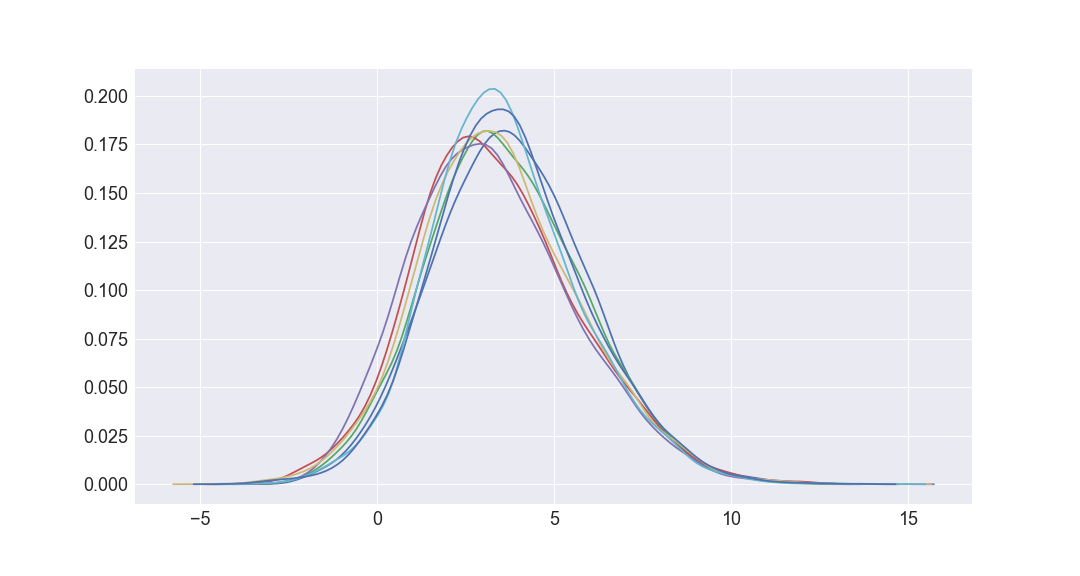
\includegraphics[width=75mm,height=40mm]{Figures/exploratory/kde_RNACru.png}&
		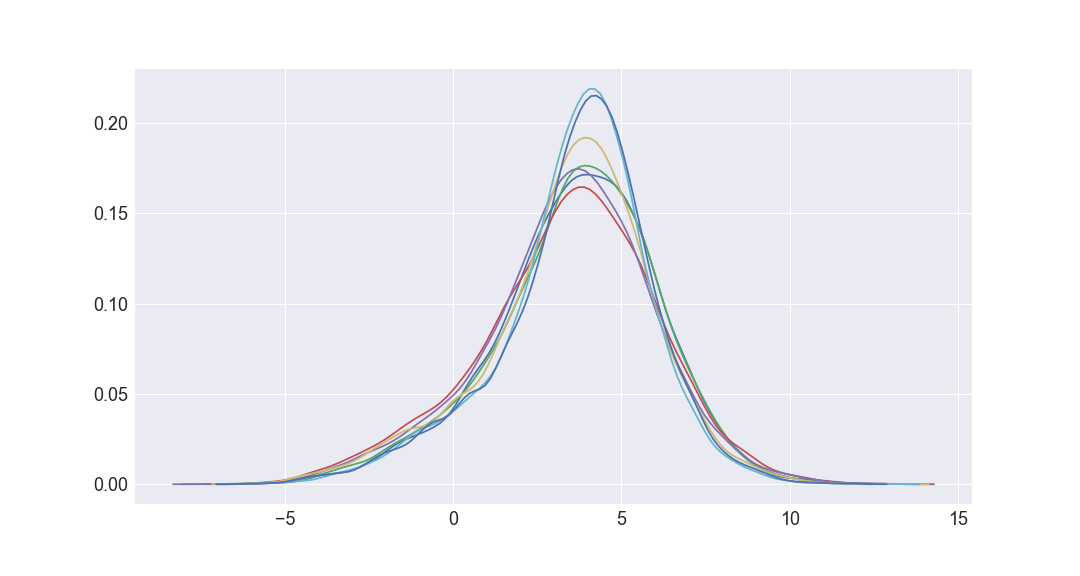
\includegraphics[width=75mm,height=40mm]{Figures/exploratory/kde_RNATot.png} \\
		RNA Crude & RNA Bulk \\
		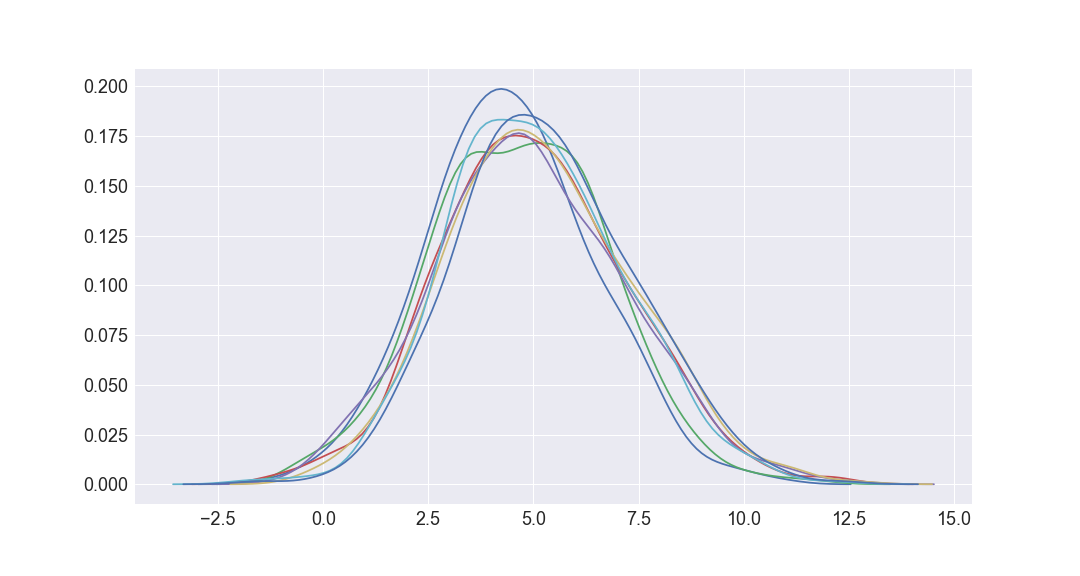
\includegraphics[width=75mm,height=40mm]{Figures/exploratory/kde_RNACruMito.png} &
		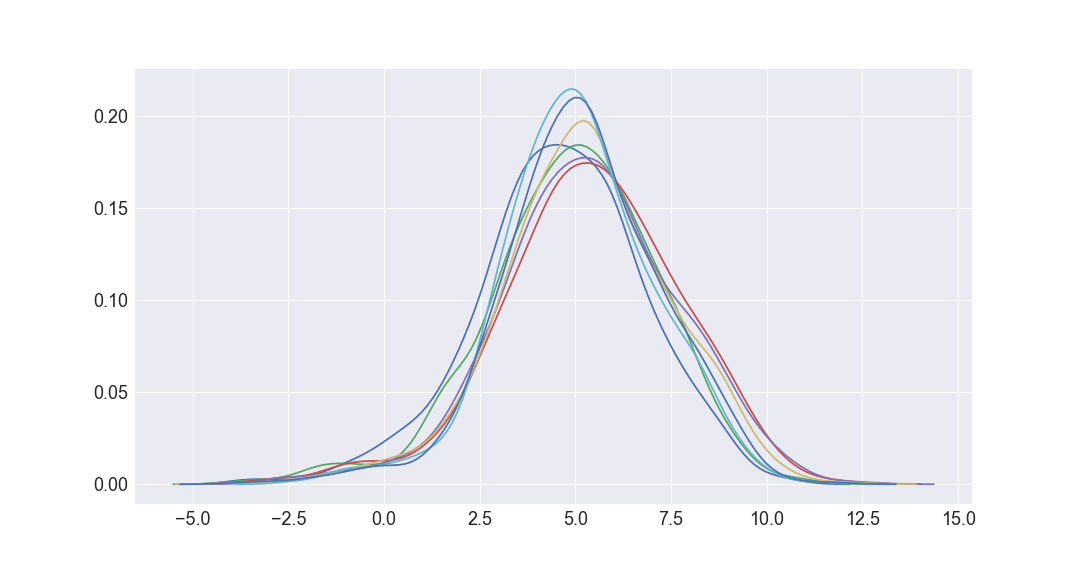
\includegraphics[width=75mm,height=40mm]{Figures/exploratory/kde_RNATotMito.png} \\
		RNA Crude Mitochondria & RNA Bulk Mitochondria
	\end{tabular}
\label{fig: KDE}
\caption{Comparison of the distribution between different datasets}
\end{figure}

\section{STEM}
\subsection{Results}
Here, we use $m=100$ and $c=3$. Using different values for $m$ and $c$ do not give us significant differences for the clustering results. We use $\delta = 0.3$ as the minimum threshold to group similar significant clusters (refer to Section \ref{3.1}). Unfortunately, STEM excludes about $40\%$ of the original pool of genes in its clustering. For RNA Crude, the number of genes considered in the significant clusters are $4894$ genes (before cluster is $8675$ genes). Similarly, for RNA Crude Mito, the number is $420$ genes (before cluster is $911$ genes). Due to this result, we decide that we only take the optimal number of clusters from STEM ($k=19$ for RNA Crude and $k=11$ for RNA Crude Mito) and then use this for the other algorithms. Moreover, we have also transformed the data into log ratios where the ratios are with respect to the expression of the first time point. We still use the original pools ($8675$ and $911$ genes for Crude and Crude Mito, respectively) of genes for the other algorithms.

%----------------------------------------------------------------------------------------

\section{Mixture Model}
\subsection{Results}
%analysis and plots
From the AIC and BIC analysis below (Figure \ref{fig: aic_bic}), we are unable to determine the optimal number of clusters as it seems that the number of clusters keeps increasing whereas from STEM, we find that the number of clusters is actually not that high. Even when we perform this analysis with maximum number of components of $>100$, we are still unable to find the optimum point. For mitochondrial genes which has at most $1000$ data, AIC and BIC analysis still could not help us extract the optimal number of clusters. The reason is probably because of the nature of the data that is not rich enough to develop obvious separable clusters (refer to \ref{2.1}). Another possible reason is that the data simply cannot be modelled as a mixture of Gaussians. As such, we initialize the number of clusters for GMM obtained from STEM and then perform GO analysis for the two covariance matrices. We then perform GO analysis on each of the resulting clusters. Nonetheless, this result may correspond to the inability of STEM to cluster most of the genes (it only clusters $\approx 60 \%$ of the total genes) which means that indeed the data can be divided into many clusters.

\begin{figure}[H]
			\centering	
	\renewcommand{\arraystretch}{0.5}
	\begin{tabular}{cc}

		\includegraphics[width=62mm,height=45mm]{Figures/opt_clust_diff0/thresh_0/RNAcruLogdiff0/RNAcru__aic_diag.png}&
		\includegraphics[width=62mm,height=45mm]{Figures/opt_clust_diff0/thresh_0/RNAcruLogdiff0/RNAcru__bic_diag.png} \\
		AIC Curve(Diagonal) & BIC Curve(Diagonal) \\
			\includegraphics[width=62mm,height=45mm]{Figures/opt_clust_diff0/thresh_0/RNAcruLogdiff0/RNAcru__aic_spherical.png}
				 &
				\includegraphics[width=62mm,height=45mm]{Figures/opt_clust_diff0/thresh_0/RNAcruLogdiff0/RNAcru__bic_spherical.png}	\\
			BIC Curve(Spherical) & BIC Curve(Spherical)  
	\end{tabular}
	\caption{AIC and BIC results for GMM with Diagonal and Spherical covariance matrices for RNA Crude data}
	\label{fig: aic_bic}
\end{figure}

%----------------------------------------------------------------------------------------

\section{K-means}
\subsection{Results}
%analysis&plots
Similar to GMM, we are unable to determine the optimum number of clusters for k-means algorithm from both the elbow curve and gap statistics analysis (Figure \ref{fig:elbowGap}). \textit{K-means} may face the same problem like GMM that the data may not be rich enough to develop separable clusters for \textit{k-means}. Another possible reasons is that euclidean distance may not be a good measure. As such, we will proceed with using optimal number of clusters obtained from STEM and the perform \textit{k-means} algorithm to the data with this initial number of clusters. Then, we perform GO analysis on the resulting clusters.

\begin{figure}[H]
	\centering
	\renewcommand{\arraystretch}{0.5}
	\begin{tabular}{cc}
		\includegraphics[width=75mm,height=45mm]{Figures/opt_clust_diff0/thresh_0/RNAcruLogdiff0/RNACru_elbow.png} &
		\includegraphics[width=75mm,height=45mm]{Figures/opt_clust_diff0/thresh_0/RNAcruLogdiff0/RNACru_gap.png} \\
		Elbow Curve(RNA Crude) & Gap Statistic Curve(RNA Crude) \\
		\includegraphics[width=75mm,height=45mm]{Figures/opt_clust_diff0/thresh_0/RNAcruMitoLogdiff0/RNACruMito_elbow.png} &				\includegraphics[width=75mm,height=45mm]{Figures/opt_clust_diff0/thresh_0/RNAcruMitoLogdiff0/RNACruMito_gap.png} \\
		Elbow Curve(RNA Crude Mito) & Gap Statistic Curve(RNA Crude Mito)
	\end{tabular}
\caption{Finding Optimal $k$ for \textit{k-means}}
\label{fig:elbowGap}
\end{figure}

%----------------------------------------------------------------------------------------

\section{Hierarchical Clustering}
\subsection{Results}
As mentioned in the previous chapter (Section \ref{4.4}), we will not be able to determine the optimal number of clusters from the dendrograms. Similar to the other algorithms, we will use $k$ obtained from STEM. In this report, we will only show the plots for HAC with Complete linkage as it gives the best results (found in Appendix \ref{AppendixA}).

%----------------------------------------------------------------------------------------
\section{Comparison of Algorithms} \label{5.2}
In this section, we use $k=19$ and $k=11$ for RNA Crude and RNA Crude Mito respectively when we apply the other clustering algorithms. From the results below (Table \ref{tab: number of genes RNA Crude} and Table \ref{tab: number of genes RNA Crude Mito}), we can see that the number of genes that fall into each cluster for different algorithms is actually quite similar (except for HAC (Comp)), especially when the total number of genes in the whole dataset is small (for RNA Crude Mito).
\begin{table}[H]
	\centering
	\begin{tabular}{lcccc}
		\hline
		\textbf{Cluster} & \textbf{K-means} & \textbf{GMM (Sph)} & \textbf{GMM (Comp)} & \textbf{HAC (Comp)} \\ \hline
		\textbf{1}       & 791              & 947                & 851                 & 2123                \\ \hline
		\textbf{2}       & 756              & 925                & 814                 & 978               \\ \hline
		\textbf{3}       & 751              & 897                & 805                 & 872                 \\ \hline
		\textbf{4}       & 678              & 720                & 712                 & 832                 \\ \hline
		\textbf{5}       & 666              & 619                & 667                 & 756                 \\ \hline
		\textbf{6}       & 658              & 554                & 636                 & 475                 \\ \hline
		\textbf{7}       & 625              & 544                & 523                 & 456                 \\ \hline
		\textbf{8}       & 573              & 480                & 503                 & 430                 \\ \hline
		\textbf{9}       & 532              & 457                & 489                 & 362                 \\ \hline
		\textbf{10}      & 492              & 455                & 473                 & 357                 \\ \hline
		\textbf{11}      & 469              & 410                & 408                 & 188                 \\ \hline
		\textbf{12}      & 460              & 355                & 376                 & 181                 \\ \hline
		\textbf{13}      & 324              & 346                & 371                 & 173                 \\ \hline
		\textbf{14}      & 276              & 243                & 334                 & 110                 \\ \hline
		\textbf{15}      & 227              & 225                & 300                 & 104                 \\ \hline
		\textbf{16}      & 178              & 212                & 175                 & 97                  \\ \hline
		\textbf{17}      & 96               & 122                & 96                  & 89                  \\ \hline
		\textbf{18}      & 69               & 100                & 82                  & 47                  \\ \hline
		\textbf{19}      & 35               & 45                 & 41                  & 45                  \\ \hline
	\end{tabular}
	\caption{Gene count in each cluster for the different algorithms \\
	($k=19$), total number of genes = $8675$}
	\label{tab: number of genes RNA Crude}
\end{table}

\begin{table}[H]
	\centering
	\begin{tabular}{lcccc}
		\hline
		\textbf{Cluster} & \textbf{K-means} & \textbf{GMM (Sph)} & \textbf{GMM (Diag)} & \textbf{HAC (Comp)}  \\ \hline
		\textbf{1}       & 134              & 140                & 121                 & 357                \\ \hline
		\textbf{2}       & 126              & 122                & 110                 & 98                 \\ \hline
		\textbf{3}       & 111              & 102                & 107                 & 84                 \\ \hline
		\textbf{4}       & 99               & 102                & 100                  & 76                   \\ \hline
		\textbf{5}       & 82               & 99                 & 100                  & 76                  \\ \hline
		\textbf{6}       & 82               & 78                 & 89                  & 69                   \\ \hline
		\textbf{7}       & 77               & 77                 & 88                  & 41                   \\ \hline
		\textbf{8}       & 69               & 57                 & 87                  & 40                  \\ \hline
		\textbf{9}       & 55               & 56                 & 56                  & 32                  \\ \hline
		\textbf{10}      & 54               & 48                 & 35                  & 28                  \\ \hline
		\textbf{11}      & 20              & 30                 & 18                  & 10                   \\ \hline
	\end{tabular}
	\caption{Gene count in each cluster for the different algorithms \\
	($k=11$), total number of genes = $911$}
	\label{tab: number of genes RNA Crude Mito}
\end{table}

\subsection{GO Analysis}
In this section, we will only show the results for RNA Crude Mito. For each of the $11$ clusters we get from the various algorithms, we perform GO analysis (we focus on \textit{biological process} (bp), \textit{cellular compartment} (cc) and \textit{KEGG pathway} (KEGG)). We use \textit{clusterprofiler} \cite{clusterprofiler} to perform our GO analysis. Our GO analysis shows that majority of the clusters indeed contain genes that share similar biological properties. This proves the earlier proposition that genes with similar biological properties may be found in the same cluster in terms of their expression values. Then, we mostly only include GO terms that are related to mitochondrial biogenesis. Furthermore, this confirms our earlier belief that traditional clustering algorithms such as GMM, K-means and HAC can still be useful in clustering time-series data, even when it is short.

When we perform GO analysis on clusters from STEM algorithm($\approx$ 50\% data) we do not get as many enriched clusters as we get from the other algorithms. This may show that STEM removes important genes that should have been clustered into one of the significant clusters. Interestingly, some enriched GO terms appear in multiple clusters, such as \textbf{mitochondrial inner membrane, OXPHOS, mitochondrial gene expression}. This means that there may be interaction between clusters. Yet, it may also be expected that these are common mitochondrially-related GO terms. By analyzing these enriched GO terms with the genes involved in each GO term further such as by incorporating additional biological data, we may then be able to make better conclusion on our objective. 

Here is a brief summary of the GO analysis for RNA Crude Mito:
\begin{itemize}
	\item K-means
	\begin{itemize}
		\item Cluster 3 (110 genes): cc (mitochondrial inner membrane, organelle inner membrane), KEGG (carbon metabolism, TCA cycle, OXPHOS)
		\item Cluster 5 (81 genes): bp (mitochondrial transport, mitochondrial gene expression), cc (mitochondrial inner membrane, mitochondrial matrix), KEGG (ribosome, OXPHOS, Parkinson's disease)		
		\item Cluster 7 (76 genes): bp (cellular respiration, mitochondrial respiratory chain complex I assembly), cc (mitochondrial inner membrane, organelle inner membrane), KEGG (OXPHOS, Parkinson's disease, Alzheimer's disease)
		\item Cluster 11 (19 genes): cc (inner mitochondrial membrane protein complex, Mitochondrial protein complext), KEGG (OXPHOS, Parkinson's disease, Thermogenesis)
	\end{itemize}
	\item GMM (Diagonal)
	\begin{itemize}
		\item Cluster 4 (99 genes): cc (mitochondrial inner membrane, organelle inner membrane, mitochondrial membrane), KEGG (OXPHOS, carbon metabolism, Huntington's diseases)
		\item Cluster 5 (99 genes): bp (mitochondrial transport, mitochondrial gene expression), cc (mitochondrial matrix, mitochondrial inner membrane, organnelle inner membrane), KEGG (OXPHOS, Thermogenesis)
		\item Cluster 6 (88 genes)8: cc (mitochondrial inner membrane, organelle inner membrane, mitochodrial protein complex), KEGG (OXPHOS, Parkinson's disease, Alzheimers' disease)
		\item Cluster 8 (86 genes): bp (mitochondrial transport, mitochondrial gene expression), cc (mitochondrial matrix, mitochondrial inner membrane)
		\item Cluster 10 (34 genes): cc (inner mitochondrial membrane, mitochondrial protein complex), KEGG (OXPHOS, Parkinson's disease, Alzheimers' disease)
	\end{itemize}
	\item GMM (Spherical)
	\begin{itemize}
		\item Cluster 3 (101 genes): cc (mitochondrial inner membrane, organelle inner membrane), KEGG (OXPHOS, carbon metabolism, Huntington's disease, Parkinson's disease)		
		\item Cluster 5 (98 genes): bp (mitochondrial transport, mitochondrial gene expression), cc (mitochondrial matrix, organelle ribosome, mitochondrial inner membrane), KEGG (ribosome, Huntington's disease)
		\item Cluster 7 (76 genes): cc (mitochondrial inner membrane, mitochondrial protein complex), KEGG (OXPHOS, Parkinson's disease, Alzheimer's disease) 
		\item Cluster 10 (47 genes): cc (mitochondrial protein complex, organelle inner membrane), KEGG (OXPHOS, Parkinson's disease, Alzheimer's disease)		
	\end{itemize}
	\item HAC (Complete)
	\begin{itemize}
		\item Cluster 1 (357 genes):  cc (mitochondrial inner membrane, organelle inner membrane), KEGG (OXPHOS, thermogenesis, carbon metabolism)
		\item Cluster 2 (98 genes): bp (purine ribonucleoside triphosphate metabolic process, ribonucleoside triphosphate metabolic process), cc (organelle inner membrane, mitochondrial inner membrane, mitochondrial matrix), KEGG (Parkinson's disease, OXPHOS)
		\item Cluster 3 (84 genes): bp (mitochondrial RNA metabolic process, mitochondrial respiratory chain complex assembly), cc (mitochondrial matrix, mitochondrial inner membrane)
		\item Cluster 4 (76 genes): bp (mitochondrial respiratory chain complex assembly, cellular respiratory), cc (mitochondrial inner membrane, organelle inner membrane), KEGG (OXPHOS, thermogenesis)
	\end{itemize}
		
\end{itemize}

Similar enriched GO terms and other terms also appear when we perform GO analysis for RNA Crude (results are exluded). The cluster plots for the above summary can be found below:

\begin{figure}[H]
	\label{fig: cluster GO plots}
	\renewcommand{\arraystretch}{0.5}
	\begin{tabular}{cccc}
		\includegraphics[width=35mm,height=30mm]{Figures/rna_cru_mito_clust_2/KMeans_cluster_8_111.png} &
		\includegraphics[width=35mm,height=30mm]{Figures/rna_cru_mito_clust_2/KMeans_cluster_4_82.png} &		
		\includegraphics[width=35mm,height=30mm]{Figures/rna_cru_mito_clust_2/KMeans_cluster_7_77.png} &		
		\includegraphics[width=35mm,height=30mm]{Figures/rna_cru_mito_clust_2/KMeans_cluster_5_20.png} \\		
		110 genes & 81 genes & 76 genes & 19 genes \\
		\includegraphics[width=35mm,height=30mm]{Figures/rna_cru_mito_clust_2/GMM-diag_cluster_5_100.png} &
		\includegraphics[width=35mm,height=30mm]{Figures/rna_cru_mito_clust_2/GMM-diag_cluster_9_100.png} &
		\includegraphics[width=35mm,height=30mm]{Figures/rna_cru_mito_clust_2/GMM-diag_cluster_8_89.png} &
		\includegraphics[width=35mm,height=30mm]{Figures/rna_cru_mito_clust_2/GMM-diag_cluster_6_35.png} \\
		99 genes & 99 genes & 88 genes & 34 genes \\
		\includegraphics[width=35mm,height=30mm]{Figures/rna_cru_mito_clust_2/GMM-sph_cluster_1_102.png} &
		\includegraphics[width=35mm,height=30mm]{Figures/rna_cru_mito_clust_2/GMM-sph_cluster_3_99.png} &		
		\includegraphics[width=35mm,height=30mm]{Figures/rna_cru_mito_clust_2/GMM-sph_cluster_6_77.png} &		
		\includegraphics[width=35mm,height=30mm]{Figures/rna_cru_mito_clust_2/GMM-sph_cluster_2_48.png} \\
		101 genes & 98 genes & 76 genes & 47 genes \\
		\includegraphics[width=35mm,height=30mm]{Figures/rna_cru_mito_clust/HAC-comp_Cluster_2_357.png} &
		\includegraphics[width=35mm,height=30mm]{Figures/rna_cru_mito_clust/HAC-comp_Cluster_3_98.png} &
		\includegraphics[width=35mm,height=30mm]{Figures/rna_cru_mito_clust/HAC-comp_Cluster_1_84.png} &
		\includegraphics[width=35mm,height=30mm]{Figures/rna_cru_mito_clust/HAC-comp_Cluster_5_76.png} \\
		357 genes & 98 genes & 84 genes & 76 genes						
	\end{tabular}
\caption{Plots comparison for the $4$ enriched clusters\\
			In order of appearance: K-means, GMM (Diagonal), GMM (Spherical), HAC (Ward)}
\end{figure}

%----------------------------------------------------------------------------------------

\section{Performance Evaluation}
In this section, we compare the performances of the different clustering algorithm with the assumption that STEM gives the optimal clustering. Here, we cannot use the whole pool of genes as STEM does not consider about half of these genes to be significant. Thus, we pick the genes that are considered significant by STEM and then apply the other clustering algorithms to these sets of genes. Then, we compare the performances of each clustering algorithm with using the two metrics described earlier (\textit{clustering accuracy} and \textit{ME distance}, refer to Section \ref{2.3}).  
\begin{table}[H]
	\centering
		\begin{tabular}{lcccccccc}
			\hline
			& \multicolumn{2}{c}{\textbf{RNA Bulk}} & \multicolumn{2}{c}{\textbf{RNA Bulk (Mito)}} & \multicolumn{2}{c}{\textbf{RNA Crude}} & \multicolumn{2}{c}{\textbf{RNA Crude (Mito)}} \\ \hline
			\textbf{Algorithm}  & \textbf{CA}       & \textbf{ME}       & \textbf{CA}           & \textbf{ME}          & \textbf{CA}        & \textbf{ME}       & \textbf{CA}           & \textbf{ME}           \\ \hline
			\textbf{K-means}    & 56.37             & 68.17             & 66.77                 & 59.91                & 48.39    & 72.60             & 45.95                 & 68.81                 \\  \hline
			\textbf{GMM (Full)} & 50.87             & 71.41             & 59.15                 & 58.84       & 51.70              & 71.00             & 53.81                 & 64.76        \\
			\textbf{GMM (Diag)} & 52.79             & 72.31             & 68.90                 & 59.15                & 44.34              & 76.24    & 42.86                 & 71.67               \\
			\textbf{GMM (Sph)}  & 57.23            & 70.55             & 66.92                 & 60.52                & 53.11              & 72.00             & 48.10                 & 67.86                 \\ \hline
			\textbf{HAC (Ward)} & 53.17             & 70.75    & 63.41                 &60.52               & 47.10              & 73.03             & 43.10                 & 71.43                 \\
			\textbf{HAC (Comp)} & \underline{71.68}    & 49.61             & \underline{78.51}        & \underline{31.55}               & \underline{67.94}              & 49.94             & \underline{71.43}       & \underline{44.76}                 \\
			\textbf{HAC (Ave)}  & 66.40             & \underline{38.88}            & 73.48                 & 33.84                & 64.73              & \underline{44.79}             & 61.43                 & \underline{44.76}                
	\end{tabular}
	\caption{Performance evaluation for the different algorithms (in \%), the underlined values are the best performing algorithm for that particular class of clustering}
	\label{tab: performance}
\end{table}

From the Table \ref{tab: performance} above, we can see that there is no algorithm that outperforms the rest for all the datasets. As expected, HAC with Complete and Average as the linkage outperforms the other algorithms since they use correlation coefficient as the distance metric just like STEM. Another interesting result is that some of the algorithms perform worse for RNA Crude (Mito) when the size of the data is smaller.